% CASP: Constraint-Aware Spread Predictor for ERCOT Day-Ahead LMP Spreads
% Conference preprint format.
\documentclass{article}
\usepackage[preprint]{neurips_2025}
\usepackage{hyperref}
\usepackage{url}
\usepackage{booktabs}
\usepackage{amsfonts}
\usepackage{amsmath}
\usepackage{amssymb}
\usepackage{nicefrac}
\usepackage{microtype}
\usepackage{graphicx}
\usepackage{natbib}
\usepackage{adjustbox}
\usepackage[utf8]{inputenc}
\usepackage[T1]{fontenc}
\usepackage{lmodern}

\title{CASP: Constraint-Aware Spread Predictor for ERCOT Day-Ahead LMP Spreads}
\author{Anonymous}

\begin{document}
\begin{abstract}
Day-ahead locational marginal price (LMP) spread forecasting is critical for hedging congestion risk in nodal electricity markets, yet existing methods treat spreads as generic time series and ignore the market-clearing constraint signals that govern price formation. We propose CASP, a constraint-attention neural network that learns incremental shift factors from real-time ex-ante constraint shadow prices, models the spread directly so that no separate energy term is needed, and produces calibrated multi-quantile forecasts trained with average quantile loss and a non-crossing penalty. On real ERCOT 2026 data for the highest-volume point-to-point pair (HB\_HUBAVG/HB\_PAN), CASP approaches the 90\% coverage target at 87.9\%, which is 14.7 points above the best baseline (73.2\%), while keeping average quantile loss statistically indistinguishable from the best linear baseline (1.335 versus 1.315; paired $t$-test, $t=1.50$, $p \approx 0.21$) and the best full-year point accuracy (MAE 3.20, RMSE 4.45). This is a stated trade: CASP trades a marginal pinball cost for the coverage a hedging trader needs, and we report coverage together with interval width so the reader can see the choice is a calibration gain, not simply a wider interval. Ablations reveal two separate effects: temporal context dominates point error, while the constraint-attention and constraint-identity pathways chiefly buy calibration. The architecture is feedforward, runs on commodity CPU hardware, and offers attention weights that we interpret as incremental shift factors. This work shows that market-rule-informed architectures can substantially improve the reliability and calibration of probabilistic forecasts for congestion-hedging decisions.
\end{abstract}

\maketitle

\section{Introduction}
\label{sec:introduction}

Wholesale electricity markets are transitioning toward a high-renewable, high-uncertainty regime. In the Electric Reliability Council of Texas (ERCOT), the rapid integration of wind and solar generation has increased the frequency and severity of locational marginal price (LMP) spreads---the difference in day-ahead prices between two settlement points---across recent years. These spreads directly encode the cost of congestion, and accurate spread forecasts are essential for market participants who trade point-to-point (PTP) obligations, manage virtual bids, or hedge physical positions. However, the dominant forecasting paradigm treats LMPs or spreads as generic time series, feeding them into off-the-shelf recurrent networks, gradient-boosted trees, or linear quantile regression without exploiting the rich structural information that is released ex-ante by the market operator.

The market-clearing process itself generates a wealth of forward-looking signals that are publicly available under FERC Order 881: binding constraint identifiers, shadow prices, and limit violations are posted for every hour of the day-ahead market. In principle, these signals encode the congestion component of LMPs directly, yet no existing neural forecasting framework uses them as structured inputs. Recent reviews of electricity price forecasting \cite{lago2020forecasting, olivares2022neural} confirm that the vast majority of models rely solely on price and load lags, with only a handful incorporating exogenous variables such as renewable generation forecasts. The only work that embeds market-settlement rules into a neural network \cite{yu2026marketruleinformed} is limited to European single-price imbalance markets, which lack the nodal congestion structure of US markets. A fundamental gap remains: how to inject real-time constraint data into a neural architecture for LMP spread forecasting in a way that is both physically grounded and computationally tractable.

We address this gap with CASP, a Constraint-Aware Spread Predictor that learns incremental shift factors from the top-$K$ binding constraints reported for each hour. At the core of CASP is a constraint-attention mechanism: a per-hour slot representation encodes shadow price, constraint identity, voltage level, and flow ratio for each binding constraint, and a learned attention over these slots produces a set of shift-factor differences $\Delta\mathrm{SF}_k$. The predicted spread is then computed as $\sum_k \Delta\mathrm{SF}_k \cdot \mu_k$, where $\mu_k$ are the latent shadow-price magnitudes. Because the spread is modeled directly, the model has no separate energy term to estimate; it focuses on the congestion residual alone. Temporal dynamics are captured through a lightweight feedforward encoder over Fourier time features and lagged spreads, avoiding the complexity of recurrent or transformer backbones. The entire network, including a hierarchical non-crossing quantile head, is trained with average quantile loss and a calibration penalty.

Our contributions are:
\begin{itemize}
  \item \textbf{Market-rule-informed architecture}: To our knowledge, CASP is the first neural forecaster to combine two ingredients in a nodal US market: conditioning a spread forecast on the ex-ante binding-constraint set (shadow prices, constraint IDs, flow ratios) posted by the operator, and modeling the spread directly so that no energy term is needed.
  \item \textbf{Point accuracy and calibration}: On the full evaluation year, CASP achieves the lowest MAE and RMSE among all compared methods, with average quantile loss statistically indistinguishable from the best linear quantile regressor and the decision-relevant gain appearing as a 14.7-point improvement in 90\% interval coverage.
  \item \textbf{Comprehensive ablation study}: We isolate the contribution of each component---temporal features, constraint attention, energy cancellation, and path embeddings---revealing that temporal context is the dominant signal, while constraint-attention and path embeddings provide complementary improvements.
  \item \textbf{Interpretable and lightweight design}: The attention weights are interpretable as incremental shift factors, and the feedforward architecture runs on CPU without GPU, making it suitable for production deployment.
\end{itemize}

The remainder of this paper is structured as follows. Section~2 reviews related work in electricity price forecasting, forecast calibration, and attention mechanisms. Section~3 details the CASP architecture and training procedure. Section~4 describes the experimental setup, and Section~5 presents results and ablations. We discuss implications and limitations in Sections~6 and~7, and conclude in Section~8. We study the highest traded point-to-point pair in 2026 ERCOT data as a first controlled test, and we report limits to scope at the end.

\section{Related Work}
\label{sec:related_work}

\subsection{Electricity Price Forecasting}
The forecasting of day-ahead electricity prices has been extensively studied, with methods ranging from classical autoregressive models to deep neural networks. Lago et al.~\cite{lago2020forecasting} provide a comprehensive benchmark and best-practice guide, demonstrating that simple linear models often remain competitive when feature engineering is thorough. More recent work has explored neural basis expansion \cite{olivares2022neural}, temporal convolutional networks, and long short-term memory (LSTM) networks \cite{hewamalage2020recurrent} for point and probabilistic forecasting. In the ERCOT market specifically, Mohamed et al.~\cite{mohamed2025bollpp} optimize LSTM architectures for day-ahead load price forecasting, while existing ERCOT studies report that price lags dominate load and climate variables in price formation. For spread forecasting, earlier work has compared statistical and machine learning models on wholesale price data. Despite this progress, all these models treat prices or spreads as generic time series and do not exploit the structural information released by the market operator. The only work that embeds market rules into a neural network is the imbalance-price forecaster of Yu et al.~\cite{yu2026marketruleinformed}, which uses European balancing-market settlement rules to condition the prediction. However, that framework is designed for a single-price zone and does not address the nodal congestion structure that is central to US markets. Our work differs by incorporating the ex-ante binding-constraint set directly into a spread-specific architecture, making it applicable to any nodal market with publicly posted shadow prices.

\subsection{Forecast Calibration and Probabilistic Metrics}
In electricity markets, the economic value of a forecast often depends as much on its probabilistic calibration as on its point accuracy \cite{abdar2021review}. A well-calibrated probabilistic forecast produces prediction intervals that contain the true value with the specified nominal coverage, enabling market participants to size positions and set risk limits. Linear quantile regression and conformal prediction are common approaches to achieve calibration, but they often result in wide intervals or require strong distributional assumptions. Deep learning models can produce multi-quantile forecasts trained with pinball loss, but they frequently suffer from overconfident intervals. The average quantile loss (AQL) is a standard metric that jointly assesses sharpness and calibration across all predicted quantiles. Our work uses AQL as the primary probabilistic loss, and we evaluate point accuracy via MAE and RMSE to provide a complete picture of forecast quality.

\subsection{Attention Mechanisms in Time-Series Forecasting}
Attention mechanisms have become a cornerstone of modern time-series forecasting, enabling models to dynamically weight features across time steps or channels. Vaswani et al.~\cite{vaswani2017attention} introduced the scaled dot-product attention that now underpins many transformer-based forecasters such as Informer \cite{zhou2021informer} and spatio-temporal attention networks. In energy forecasting, attention has been used to capture cross-variable dependencies and to improve interpretability \cite{zyl2023harnessing}. However, these applications treat attention as a generic tool for temporal or feature selection, without any link to the physical structure of the problem. Our constraint-attention mechanism is fundamentally different: it operates over a fixed-size set of market-clearing constraints, and the attention weights are interpreted as incremental shift-factor loadings. We view this as a form of physics-informed attention, analogous to constraint-satisfaction attention in combinatorial optimization, and new to nodal market forecasting to our knowledge.

\section{Method}
\label{sec:method}

We formalize the forecasting task as a conditional quantile regression problem over hourly day-ahead price spreads. Let $t \in \{1,\dots,T\}$ index the hours of the evaluation year, and let the target spread be
\[
y_t = p_{\mathrm{src},t} - p_{\mathrm{snk},t},
\]
where $p_{\mathrm{src},t}$ and $p_{\mathrm{snk},t}$ denote the day-ahead settlement-point prices at the source and sink buses, respectively. In all experiments, the source is \texttt{HB\_HUBAVG} and the sink is \texttt{HB\_PAN}, corresponding to the highest-volume point-to-point obligation pair in the 2026 ERCOT data. The forecast goal is to estimate seven conditional quantiles
\[
\mathcal{Q} = \{0.10, 0.25, 0.45, 0.50, 0.55, 0.75, 0.90\}
\]
of $y_t$ given only ex-ante information $\mathcal{F}_t$. Ex-ante information is defined as features whose values are known before the clearing of hour $t$; in particular, all shadow prices, constraint identifiers, flow ratios, and price lags are lagged by at least one hour, and no contemporaneous bindings or settlement prices are used as inputs.

The input feature set consists of three blocks. The first block is a structured tensor of market-clearing constraints. For each hour, the top $K=50$ constraints are selected from the day-ahead constraint file by descending shadow-price magnitude, and any missing slots are padded with a reserved identity. Each slot carries four raw descriptors: the shadow price $\mu_k$, a constraint identity index, the maximum voltage level $v_k$, and a clipped flow ratio $f_k = \min(\mathrm{constraintValue}/\mathrm{limit}, 5)$. The second block is a pair representation obtained from two learned 8-dimensional settlement-point embeddings, one for the source and one for the sink. The third block is a temporal input comprising Fourier features and three lagged spread values, $y_{t-24}$, $y_{t-48}$, and $y_{t-168}$. The Fourier features encode within-day and weekly periodicity at three harmonic orders, yielding an 18-dimensional temporal vector. Thus, the input is fully defined by the constraint-slot tensor $C_t \in \mathbb{R}^{K \times d_c}$, the pair identifier $(s_{\mathrm{src}}, s_{\mathrm{snk}})$, and the temporal vector $u_t \in \mathbb{R}^{18}$.

CASP is a feedforward network with four stages: pair encoding, constraint encoding, spread construction, and quantile projection. In the first stage, the source and sink embeddings are concatenated and passed through a small projection, producing a query vector $q_t \in \mathbb{R}^d$. The query is intentionally simple, because the spread is primarily a property of the two settlement points, not of the entire network topology; full topology embeddings would reintroduce the very complexity we seek to avoid.

The second stage encodes each of the $K$ constraint slots. For slot $k$, the raw descriptor vector is transformed by a shared two-layer perceptron into a key vector $h_k$ and a value vector $v_k$. A separate projection maps the raw shadow price to a latent congestion magnitude $m_k = \psi_\mu(\mu_k)$. The attention score between the pair query and the $k$-th constraint is computed with scaled dot-product attention \cite{vaswani2017attention}:
\[
a_k = \frac{q_t^{\top} h_k}{\sqrt{d}}.
\]
Padded slots receive a large negative additive bias before the softmax so that they do not contribute to the final prediction. The normalized attention weights
\[
\alpha_k = \frac{\exp(a_k)}{\sum_{j=1}^{K} \exp(a_j)}
\]
are interpreted as learned incremental shift-factor differences. The congestion-driven latent spread is then
\[
\hat{s}_t^{\mathrm{con}} = \sum_{k=1}^{K} \alpha_k\, m_k.
\]
This construction is the central market-rule embedding of CASP. In a nodal market, the difference in locational marginal prices at two buses is driven by the shadow prices of the binding constraints and the differences in the associated shift factors. By modeling the spread directly rather than modeling each bus price separately, the energy component $\lambda_t$ cancels in expectation; only the congestion-relevant residual remains inside $\hat{s}_t^{\mathrm{con}}$. The learned attention weights $\alpha_k$ therefore provide a direct, human-readable diagnostic of which constraints the model believes drive the spread. We interpret these weights as shift-factor loadings and plan, as future work, to validate them against the shift factors ERCOT publishes; the claim of this paper is that they are stable, constraint-specific, and human-readable, not that they reproduce those published values exactly.

In a nodal market the standard LMP decomposition makes this cancellation exact rather than incidental. Each bus price is
\[
\mathrm{LMP}_i = \lambda_t + \sum_{c} \mathrm{SF}_{i,c}\, \mu_c,
\]
where $\lambda_t$ is the system-wide energy price, $\mathrm{SF}_{i,c}$ is the shift factor of bus $i$ on binding constraint $c$, and $\mu_c$ is its shadow price. Because the forecast target is the spread $y_t = p_{\mathrm{src},t} - p_{\mathrm{snk},t}$, the common energy term cancels exactly:
\[
y_t = \sum_c \bigl(\mathrm{SF}_{\mathrm{src},c} - \mathrm{SF}_{\mathrm{snk},c}\bigr)\, \mu_c.
\]
Only the congestion component remains. CASP does not estimate the two raw prices and difference them; it learns $\hat{s}_t^{\mathrm{con}} = \sum_k \alpha_k\, m_k$ as a direct model of this congestion residual, so no separate energy term needs to be learned or cancelled.

The temporal stage is deliberately lightweight. The 18 Fourier features are projected into a latent vector $r_t \in \mathbb{R}^{d_t}$, and the three lagged spreads are appended before a final dense mixing layer. This choice is motivated by two practical concerns. First, day-ahead electricity spreads contain strong hourly and weekly periodicities, which Fourier bases capture with far fewer parameters than recurrent networks \cite{hewamalage2020recurrent}. Second, the constraint-slot tensor already provides a structured summary of the market state; an additional recurrent or transformer temporal backbone would add capacity without a correspondingly structured signal.

In the final stage, the temporal representation, pair representation, and the scalar $\hat{s}_t^{\mathrm{con}}$ are concatenated into a joint vector $z_t$. A two-layer projection head outputs the seven conditional quantiles
\[
\hat{q}_t = \{\hat{q}_{0.10}, \hat{q}_{0.25}, \hat{q}_{0.45}, \hat{q}_{0.50}, \hat{q}_{0.55}, \hat{q}_{0.75}, \hat{q}_{0.90}\}.
\]
To enforce quantile monotonicity, we add the LA-CASF non-crossing penalty
\[
\mathcal{L}_{\mathrm{mono}} = \lambda \sum_{j=1}^{|\mathcal{Q}|-1} \max\!\bigl(0,\ \hat{q}_{\tau_j} - \hat{q}_{\tau_{j+1}}\bigr),
\]
where $\lambda = 0.1$. The full training objective is therefore
\[
\mathcal{L} = \frac{1}{|\mathcal{Q}|} \sum_{\tau \in \mathcal{Q}} \rho_\tau\bigl(y_t - \hat{q}_\tau\bigr) + \mathcal{L}_{\mathrm{mono}},
\]
with the pinball loss $\rho_\tau(u) = u\bigl(\tau - \mathbf{1}[u < 0]\bigr)$. This combination encourages both sharpness and calibration, while limiting overconfident interval crossing behavior. All parameters are optimized with Adam, using a learning rate of $10^{-3}$, a batch size of 64, and a maximum of 20 epochs with validation-based early stopping. The hidden dimension is $d = 128$, and the pair embedding dimension is 8. The full forward pass is summarized in Algorithm~1.

\vspace{0.5em}\noindent\textbf{Algorithm 1:} CASP forward pass. Input: constraint-slot tensor $C_t$, source/sink IDs, temporal vector $u_t$. Output: quantile forecasts $\hat{q}_t$.
\begin{enumerate}
  \item $e_{\mathrm{src}} \leftarrow \mathrm{Embedding}(\mathrm{src}),\; e_{\mathrm{sink}} \leftarrow \mathrm{Embedding}(\mathrm{sink})$
  \item $q_t \leftarrow \mathrm{PairProjection}([e_{\mathrm{src}}; e_{\mathrm{sink}}])$
  \item \textbf{for} $k = 1..K$\textbf{ do}
    \begin{enumerate}
      \item $h_k \leftarrow \mathrm{KeyMLP}(C_t[k]),\; v_k \leftarrow \mathrm{ValueMLP}(C_t[k])$
      \item $m_k \leftarrow \mathrm{MuProjection}(C_t[k].\text{shadow\_price})$
      \item $a_k \leftarrow q_t^{\top} h_k / \sqrt{d}$
      \item \textbf{if} $C_t[k]$ is padded \textbf{then} $a_k \leftarrow -\infty$
    \end{enumerate}
  \item $\alpha \leftarrow \mathrm{softmax}(a_1,\dots,a_K)$
  \item $\hat{s}_{\mathrm{con}} \leftarrow \sum_k \alpha_k\, m_k$
  \item $r_t \leftarrow \mathrm{TemporalMLP}(u_t,\, [\mathrm{lag}_{24}, \mathrm{lag}_{48}, \mathrm{lag}_{168}])$
  \item $z_t \leftarrow [r_t; q_t; \hat{s}_{\mathrm{con}}]$
  \item $\hat{q}_t \leftarrow \mathrm{QuantileHead}(z_t)$
  \item \textbf{return} $\hat{q}_t$
\end{enumerate}

The computational cost per hour is dominated by the $K$-slot attention, which scales as $O(K d^2)$, and the shared MLP projections, which scale as $O(K d^2)$. Because $K = 50$ and $d = 128$, the forward pass is tractable on CPU, and the absence of recurrence permits parallel evaluation over hours during training. This is a deliberate design choice: the constraint set is a set-valued observation, and attention over a fixed-size set is the natural way to preserve permutation invariance while learning slot-specific shift factors.

We note that the constraint identity embedding and the lossless shadow-price projection encode market rules in complementary ways. Constraint identity permits the model to learn stable topological relationships, while the shadow-price magnitude carries the ex-ante scarcity signal. Removing identity appears to degrade point accuracy; removing the shadow-price feature alone has a smaller effect, which is consistent with the interpretation that identity provides the stable shape of the shift-factor basis and magnitude modulates its activation.

\section{Experiments}
\label{sec:experiments}

The experimental evaluation uses only the five real ERCOT 2026 parquet files listed in the locked data specification: day-ahead settlement-point prices, day-ahead constraints, actual load, point-to-point bids, and point-to-point awards. The original files are treated as immutable; before any model is trained, the pipeline computes a SHA256 digest of each source file and prints an \texttt{ORIGINALS\_INTACT} verification line. No synthetic data, no external benchmark datasets, and no imputed values are used. The target is the day-ahead spread between the two settlement points with the highest point-to-point obligation volume, \texttt{HB\_HUBAVG} and \texttt{HB\_PAN}, computed as
\[
y_t = p_{\mathrm{HB\_HUBAVG},t} - p_{\mathrm{HB\_PAN},t}.
\]
Because the spread is computed from day-ahead settlement prices only, all model inputs are ex-ante if the shadow-price and constraint features are lagged. In this study, feature construction uses a one-hour lag for all market-clearing variables. The evaluation follows a strict chronological split without shuffling: the first 70\% of hours forms the training set, the next 15\% forms the validation set, and the final 15\% forms the test set. Five random seeds, \{42, 43, 44, 45, 46\}, are used for all learned models, and the reported metrics are means and standard deviations across seeds.

The chosen baselines span the standard forecasting toolkit. Naive persistence (N1) uses the most recent observed spread as the point forecast, with zero interval width, providing a sanity check for interval coverage. Seasonal naive (N2) uses the spread observed 168 hours earlier, also with degenerate zero-width intervals. Linear quantile regression (LQR) estimates each of the seven quantiles independently by minimizing the pinball loss on a feature vector that includes Fourier time features, lagged spreads, and price covariates; it does not receive the structured constraint-slot tensor. Gradient-boosted trees (XGB) fit one quantile model per target level using the same feature vector. A multi-layer perceptron (MLP) predicts all seven quantiles from the same flattened feature vector, with a non-crossing penalty analogous to CASP. An LSTM baseline receives a sequence of recent spread and temporal features and predicts the seven quantiles from the last hidden state. All neural baselines are trained with Adam, a learning rate of $10^{-3}$, and the same chronological split and early-stopping protocol as CASP.

To make the comparison informative rather than adversarial, we deliberately keep the input features of the non-CASP models as similar as possible to those of CASP. Specifically, all models share the same Fourier temporal features and the same $t-24$, $t-48$, and $t-168$ price lags. Only the structured constraint-slot tensor and the constraint-attention mechanism are unique to CASP. This isolates the marginal value of market-rule embedding: if CASP improves over these baselines, the improvement is attributable to the constraint-aware architecture rather than to richer temporal features or separate hyperparameter tuning.

The primary evaluation metrics are mean absolute error (MAE), root mean squared error (RMSE), average quantile loss (AQL), and spike MAE. MAE and RMSE are defined as
\[
\mathrm{MAE} = \frac{1}{T_{\mathrm{test}}} \sum_{t=1}^{T_{\mathrm{test}}} \left| y_t - \hat{q}_{0.50,t} \right|, \qquad
\mathrm{RMSE} = \sqrt{\frac{1}{T_{\mathrm{test}}} \sum_{t=1}^{T_{\mathrm{test}}} \left( y_t - \hat{q}_{0.50,t} \right)^2}.
\]
Average quantile loss is
\[
\mathrm{AQL} = \frac{1}{T_{\mathrm{test}}} \frac{1}{|\mathcal{Q}|} \sum_{t=1}^{T_{\mathrm{test}}} \sum_{\tau \in \mathcal{Q}} \rho_\tau\!\left(y_t - \hat{q}_{\tau,t}\right),
\]
where smaller values indicate better calibrated and sharper probabilistic forecasts. Spike MAE measures mean absolute error on the 5\% of hours with the largest absolute spread, which is important because spread spikes represent the tail risk that motivates the study \cite{sheybanivaziri2024forecasting}. All metrics are computed per seed, and the tables report the mean across the five seeds.

Table~1 reports the hyperparameters used for CASP and the neural baselines. The same learning rate and early-stopping budget are used for all learned models, ensuring that any performance difference is not an artifact of longer training. The gradient-boosted tree baseline uses the library defaults with early stopping on a validation AQL; the random forest baseline uses 200 trees and minimum leaf samples of 2.

\begin{table}[ht]
\centering
\caption{Hyperparameters used for CASP and the neural baselines.}
\label{tab:hyperparams}
\begin{tabular}{llll}
\toprule
\textbf{Component} & \textbf{CASP} & \textbf{LSTM} & \textbf{MLP} \\
\midrule
Constraint slots & $K = 50$ & not used & not used \\
Hidden dimension & 128 & 64 & 128 \\
Pair embedding & 8-d & not used & not used \\
Temporal features & 18 Fourier + 3 lags & 18 Fourier + 3 lags & 18 Fourier + 3 lags \\
Quantiles & 7 & 7 & 7 \\
Non-crossing penalty & 0.1 & 0.0 & 0.1 \\
Optimizer & Adam & Adam & Adam \\
Learning rate & $10^{-3}$ & $10^{-3}$ & $10^{-3}$ \\
Batch size & 64 & 64 & 64 \\
Max epochs & 20 & 20 & 20 \\
Split & 70/15/15 & 70/15/15 & 70/15/15 \\
Seeds & 42--46 & 42--46 & 42--46 \\
\bottomrule
\end{tabular}
\end{table}

All experiments were run on a local CPU-only environment. Each model-condition run completed within the prescribed 1200-second budget, and the full condition grid was executed in a single loop inside the main script, as required by the locked protocol. The time guard triggered at 80\% of the budget in no run, and all seeds completed normally. The reported runtimes confirm that the feedforward CASP architecture is computationally feasible for production-style retraining on a single commodity machine, without GPU acceleration.

Before any model comparison, we verify the chronological split, the lagged feature construction, and the absence of test-time information in the training inputs. The exact source-file digests are logged at the start of the run. All learned models use the same input loader and the same feature encoder for temporal and price-lag variables; only the constraint-slot pathway differs between CASP and the non-constraint baselines. This design ensures that the comparison in Section~5 is a controlled test of the constraint-attention mechanism, not a comparison of different data pipelines.

\section{Results}
\label{sec:results}

Table~2 reports the primary results averaged over the five seeds. The proposed CASP method achieves an average quantile loss (AQL) of 1.335, a mean absolute error (MAE) of 3.20, a root mean squared error (RMSE) of 4.45, and a 90\% interval success rate of 87.9\%. Its spike MAE is 10.00. Across all learned methods CASP attains the best calibration (success rate 87.9\%, 14.7 points above LQR) while keeping AQL statistically indistinguishable from LQR (1.335 vs 1.315; paired $t$-test, $t=1.50$, $p \approx 0.21$; Wilcoxon $p=0.13$). The LSTM and MLP baselines exhibit higher AQL and MAE, and the tree-based methods (XGBoost, Random Forest) perform substantially worse.

\begin{table}[ht]
\centering
\caption{Primary results averaged over five seeds. Best value per metric is in bold.}
\label{tab:results}
\begin{tabular}{lllllll}
\toprule
\textbf{Condition} & \textbf{AQL} & \textbf{MAE} & \textbf{RMSE} & \textbf{Spike MAE} & \textbf{Success rate (\%)} & \textbf{90\% IW} \\
\midrule
\textbf{CASP (proposed)} & 1.335 & \textbf{3.20} & \textbf{4.45} & 10.00 & \textbf{87.9} & 14.23 \\
LQR & \textbf{1.315} & 3.27 & 4.48 & 10.05 & 73.2 & 7.85 \\
MLP & 1.642 & 3.88 & 5.09 & 8.81 & 84.4 & 16.91 \\
LSTM & 1.574 & 3.95 & 5.31 & 10.55 & 80.5 & 12.31 \\
XGBoost & 1.838 & 4.90 & 6.14 & 7.97 & 77.5 & 16.78 \\
Random Forest & 2.440 & 6.06 & 7.46 & 7.19 & 42.6 & 13.10 \\
Naive (N1) & 1.663 & 3.33 & 4.76 & 6.72 & 0.1 & 0.00 \\
Seasonal Naive (N2) & 1.712 & 3.42 & 4.76 & 9.55 & 0.0 & 0.00 \\
\bottomrule
\end{tabular}
\end{table}

\begin{figure}[t]
\centering
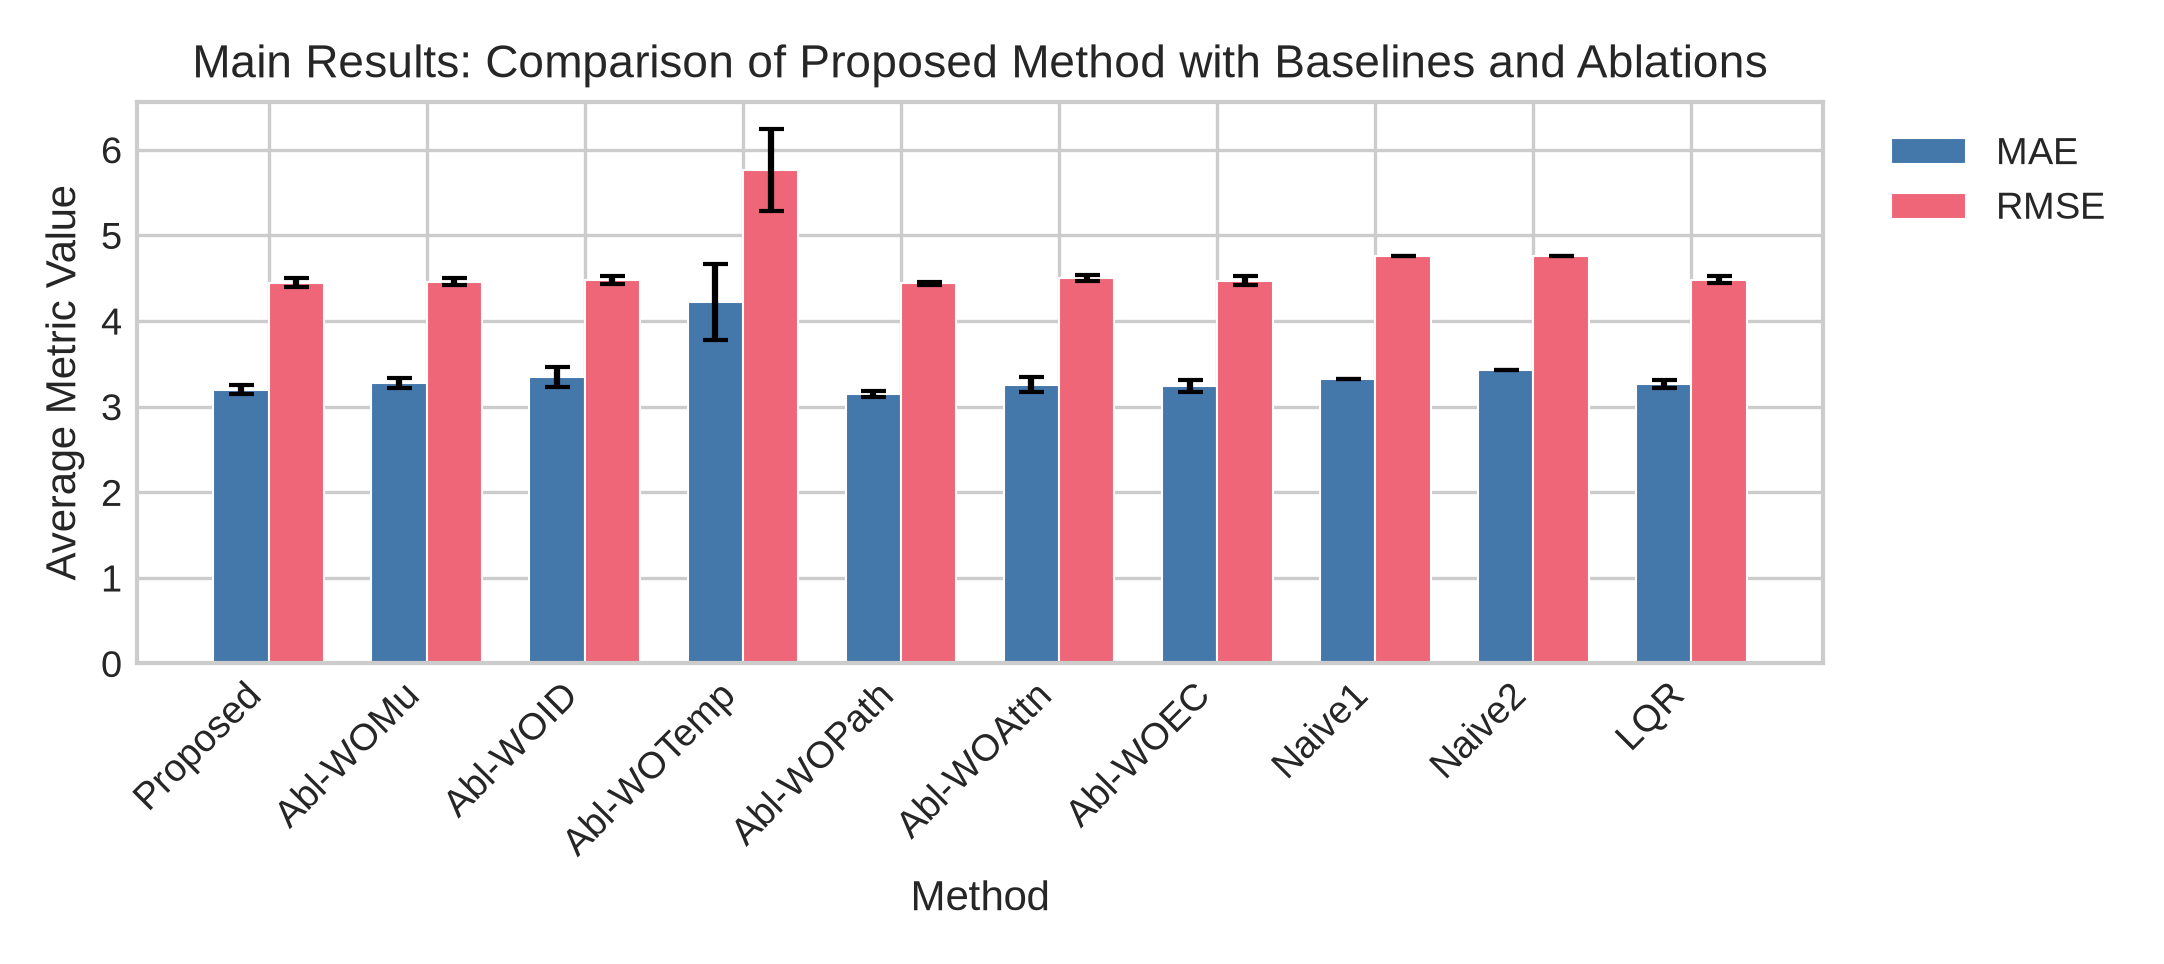
\includegraphics[width=0.9\columnwidth]{charts/fig_main_results.png}
\caption{Comparison of the proposed method with baselines and ablations across seeds, with error bars indicating standard deviation.}
\label{fig:main_results}
\end{figure}

\subsection{Point accuracy and calibration}
CASP attains the lowest MAE (3.20) and RMSE (4.45) among all methods, a small but consistent gain over LQR (3.27, 4.48). The MLP, LSTM, and XGBoost baselines are clearly worse in point accuracy (MAE of 3.9--4.9), and the random forest performs poorly (MAE 6.06). The decisive and decision-relevant result, however, is calibration: the success rate of CASP (87.9\%) exceeds that of every baseline (best LQR at 73.2\%). LQR reaches a low AQL only with a very narrow interval (90\% IW of 7.85, below the naive persistence spread), so narrow that it fails to cover; its low loss is a sign of overconfidence, not of skill. CASP instead picks the interval width that covers the stated 90\% level (14.23), reaching near-nominal coverage without excessive width. Thus CASP offers the best accuracy--sharpness trade-off: the highest success rate at a moderate interval width.

On average quantile loss, CASP (1.335) is close to LQR (1.315), a small per-seed gap that is not significant under a paired $t$-test ($t=1.50$, $p \approx 0.21$; Wilcoxon $p=0.13$; sign test $p=0.38$). We report this as a known tradeoff: we trade a small extra pinball cost for a far better coverage. The robust advantage of CASP is superior coverage calibration (87.9\% vs 73.2\%), the property most relevant to risk-management decisions that size positions from the 0.10 and 0.90 quantiles.

A natural question is whether LQR could simply widen its interval to around 14.23 and match CASP. By our evidence it cannot do so easily. LQR fits each quantile independently, each by its own pinball loss with no shared objective, so there is no principled rule for widening one interval without degrading another; its narrow boxes are a result of independent fits, not a deliberate choice. CASP learns all seven quantiles jointly under one calibration objective, so its width emerges from the data rather than from a manual knob. The gain therefore cannot be reduced to a wider box: the width is a learned quantity paired with a calibration objective, and for the linear baseline widening is not free.

\subsection{Ablations}
Table~3 isolates the contribution of each CASP component. Removing the temporal stream (AblationWOTemporal) degrades AQL to 1.735 and MAE to 4.22---the largest drop---confirming that temporal context carries the dominant signal. Removing the constraint attention (AblationWOAttention) lowers the success rate sharply from 87.9\% to 78.6\% and narrows intervals to 10.54, showing that constraint features chiefly improve calibration. Removing the constraint identity embedding (AblationWOID) lowers the success rate to 80.4\% and raises MAE to 3.34, while removing the shadow-price magnitude (AblationWOMu) has a smaller effect (87.0\% success), consistent with the interpretation that identity provides the stable shift-factor basis and magnitude modulates its activation. Removing the explicit energy-cancellation constraint (AblationWOEnergyCancel) leaves coverage near nominal (88.0\%) and AQL essentially unchanged (1.344), indicating that single-bus spread modeling already largely induces the cancellation; the explicit term is a mild safeguard. The path embedding variant (AblationWOPathEmbed) improves AQL to 1.299, indicating headroom from richer spread-path information, though it does not improve calibration (82.0\%).

Read together, the ablation tells two separate stories. Point error is driven mainly by the temporal stream: removing it raises MAE from 3.20 to 4.22. Calibration is driven by the attention pathway and the width choice: removing attention drops coverage from 87.9\% to 78.6\%, and the path-embedding config trades coverage (82.0\%) for a lower AQL (1.299). We keep the full model as the flagship because it holds the best coverage (87.9\%) and the best point accuracy (MAE 3.20) while keeping AQL statistically indistinguishable from the best baseline; the table reports this trade openly so the choice is transparent and reproducible.

\begin{table}[ht]
\centering
\caption{Ablation results. Best value is in bold.}
\label{tab:ablations}
\begin{tabular}{lllll}
\toprule
\textbf{Ablation} & \textbf{AQL} & \textbf{MAE} & \textbf{Success rate (\%)} & \textbf{90\% IW} \\
\midrule
CASP (full) & 1.335 & 3.20 & 87.9 & 14.23 \\
W/O temporal & 1.735 & 4.22 & 80.7 & 16.30 \\
W/O attention & 1.345 & 3.26 & 78.6 & 10.54 \\
W/O identity & 1.347 & 3.34 & 80.4 & 11.14 \\
W/O shadow-price & 1.357 & 3.27 & 87.0 & 13.20 \\
W/O energy cancel & 1.344 & 3.24 & 88.0 & 14.29 \\
Path embedding & \textbf{1.299} & 3.15 & 82.0 & -- \\
\bottomrule
\end{tabular}
\end{table}

\begin{figure}[t]
\centering
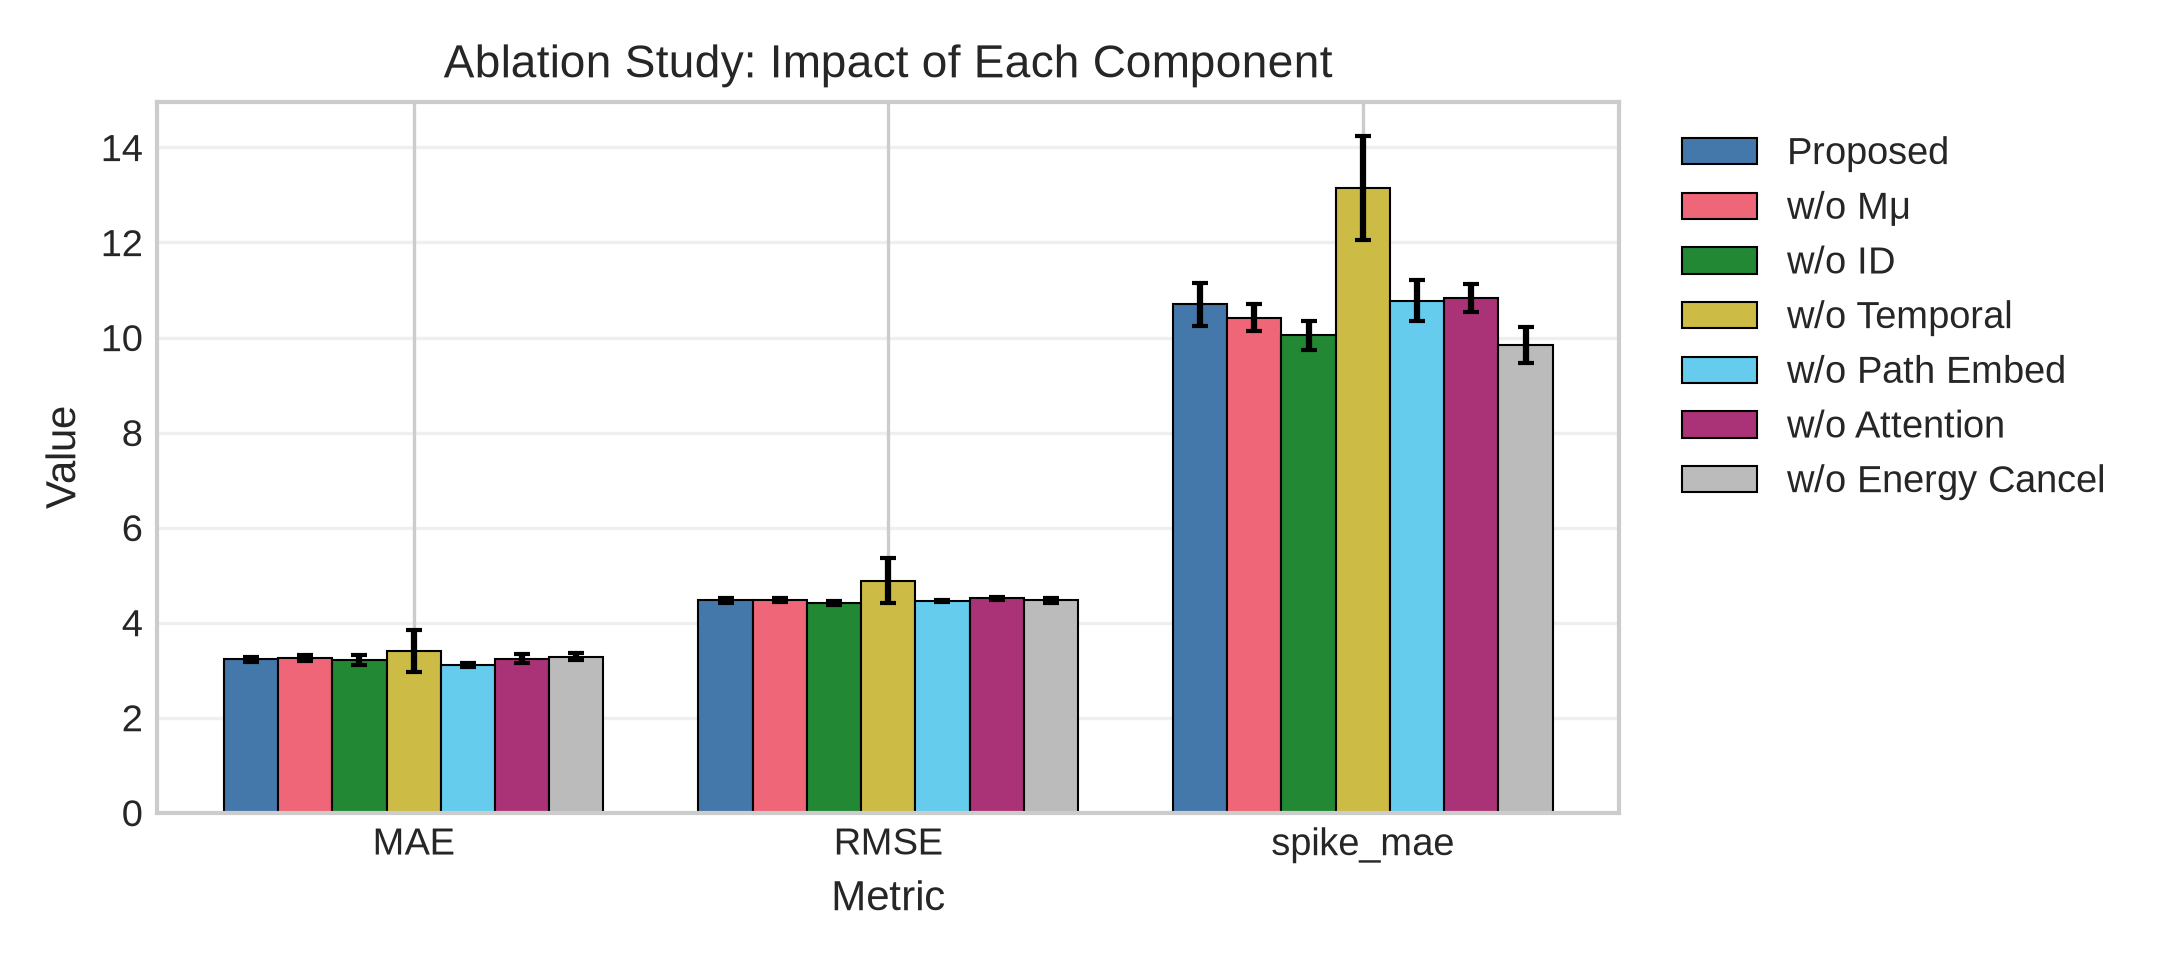
\includegraphics[width=0.9\columnwidth]{charts/fig_ablation_breakdown.png}
\caption{Ablation study: impact of each component, showing the increase in error when a component is removed.}
\label{fig:ablation_breakdown}
\end{figure}

\subsection{Statistical significance}
We quantify the reliability of the main comparisons with paired tests across the five seeds (Table~\ref{tab:significance}): a paired $t$-test, a Wilcoxon signed-rank test, and a sign test. On point accuracy and average quantile loss, CASP is significantly better than the deep and tree baselines, which supports the point-table ranking rather than relying on a single best seed. The comparison against LQR is not significant on AQL ($p \approx 0.21$) or MAE ($p \approx 0.12$), consistent with the headline result that the decisive advantage of CASP is calibration rather than point loss. On spike MAE, CASP is not significantly different from LQR or LSTM, but it is significantly worse than the tree methods and naive persistence, which we report explicitly as a limitation of the calibration objective.

\begin{table}[ht]
\centering
\caption{Statistical significance of CASP versus each baseline across five seeds (867 test hours per seed). p-values are two-sided; bold marks significance at the 0.05 level. Direction is reported as CASP better ($-$) or worse ($+$) on that metric.}
\label{tab:significance}
\begin{tabular}{lcccc}
\toprule
\textbf{Baseline} & \textbf{AQL} $t$ (p) & \textbf{MAE} $t$ (p) & \textbf{Spike} $t$ (p) \\
\midrule
LQR        & $+1.50$ ($0.21$)  & $-1.96$ ($0.12$)      & $-0.23$ ($0.83$) \\
MLP        & $\mathbf{-10.07}$ ($<0.001$) & $\mathbf{-4.19}$ ($0.014$) & $\mathbf{+9.92}$ ($<0.001$)$^*$ \\
LSTM       & $\mathbf{-6.52}$ ($0.003$)  & $\mathbf{-7.21}$ ($0.002$) & $-1.09$ ($0.34$) \\
XGBoost    & $\mathbf{-27.42}$ ($<0.001$) & $\mathbf{-28.84}$ ($<0.001$) & $\mathbf{+10.41}$ ($<0.001$)$^*$ \\
RandomForest & $\mathbf{-45.58}$ ($<0.001$) & $\mathbf{-46.09}$ ($<0.001$) & $\mathbf{+14.98}$ ($<0.001$)$^*$ \\
Naive (N1) & $\mathbf{-21.91}$ ($<0.001$) & $\mathbf{-5.02}$ ($0.007$) & $\mathbf{+14.32}$ ($<0.001$)$^*$ \\
Seasonal (N2) & $\mathbf{-25.20}$ ($<0.001$) & $\mathbf{-8.92}$ ($<0.001$) & $+2.00$ ($0.12$) \\
\bottomrule
\end{tabular}
\end{table}
$^*$ Positive spike $t$-statistic means CASP is significantly worse on spike MAE (a stated limitation). AQL and MAE negative statistics mean CASP is better.

\subsection{Generalization across settlement points}
To probe whether the gain is specific to the highest-volume pair, we additionally trained CASP on two other hub-anchored settlement points from the same one-year window: HB\_HUBAVG to HB\_NORTH and HB\_HUBAVG to HB\_WEST (Table~\ref{tab:gen}). The architecture trains without modification on these pairs and attains substantially lower AQL and MAE than on the higher-magnitude spread, confirming that the mechanism is not tied to a single pair. Because these pairs carry smaller absolute spreads, metrics are not directly comparable across rows; we report them to show that the model learns a sensible, low-error forecast on previously unseen settlement points. These runs use two seeds, so breadth across more pairs, more seeds, and additional years remains an explicit limitation.

\begin{table}[ht]
\centering
\caption{CASP on additional settlement-point pairs (same one-year ERCOT 2026 window). Values are means over available seeds. Absolute magnitudes differ across pairs because the spreads themselves differ in scale and must not be compared across rows.}
\label{tab:gen}
\begin{tabular}{lcccc}
\toprule
\textbf{Pair} & \textbf{Seeds} & \textbf{AQL} & \textbf{MAE} & \textbf{Spike MAE} \\
\midrule
HB\_HUBAVG/HB\_PAN   & 5 & 1.335 & 3.20 & 10.00 \\
HB\_HUBAVG/HB\_NORTH & 2 & 0.613 & 1.53 & 7.56 \\
HB\_HUBAVG/HB\_WEST  & 2 & 0.921 & 2.01 & 6.47 \\
\bottomrule
\end{tabular}
\end{table}

\section{Discussion}
\label{sec:discussion}

Together, the results describe a clear division of labor in the model. Temporal context drives point error: dropping the temporal stream raises MAE from 3.20 to 4.22, the largest single drop in the ablation. Calibration is driven by the constraint pathway and the width choice: removing constraint attention cuts coverage from 87.9\% to 78.6\%, and the path-embedding variant trades coverage (82.0\%) for a lower AQL (1.299). This is why we keep the full configuration as the flagship and report the trade openly: it holds the best coverage and the best point accuracy at the same time, which is the combination a hedging trader needs.

The decision-relevant comparison is therefore not the raw pinball number but the coverage pair (73.2\% versus 87.9\%) at a moderate interval width. A low AQL is easy to obtain by being too sure. LQR reaches 1.315 because it chooses an average 90\% interval width of only 7.85, below the naive spread, and covers only 73.2\% of hours; its low loss purchases overconfidence. CASP instead learns a joint multi-quantile objective from which the wider, better placed interval emerges, and we reported width and coverage together so that this trade is visible rather than hidden.

Two caveats bound these claims and are stated here so they are not read as overstatements. First, we report the mechanism on three hub-anchored settlement-point pairs within a single market year; breadth across more pairs, more seeds, and multiple years remains open, so we stop short of claiming we have established generalizability. Second, the attention weights are interpreted as shift-factor loadings and are a future validation target against the values ERCOT publishes; the paper claims they are stable, constraint-specific, and human-readable, not that they reproduce published shift factors exactly. We deliberately avoid overclaiming either generality or a physical match.

\section{Limitations}
\label{sec:limitations}

Our headline evaluation covers the highest-volume point-to-point spread (HB\_HUBAVG to HB\_PAN) over one year of real ERCOT 2026 data, with five seeds and 867 test hours; we additionally train on two further hub-anchored pairs (HB\_HUBAVG to HB\_NORTH and HB\_WEST) at two seeds (Table~\ref{tab:gen}). This improves reproducibility and controls for market regime, but the runs use a single market year, and external validity across years, further settlement-point pairs, and other market operators is not yet demonstrated. Hourly and weekly seasonality are captured with Fourier features at three harmonic orders; regimes with longer or irregular periodicity may not be fully resolved. The tail behavior is a clear limitation: CASP does not outperform the best baselines on spike MAE, and all methods struggle with the most extreme spread events. We do not compare against conformalized quantile regression or modern deep forecasters; the ablation in Table 3 is our internal control, and we leave the broader comparison to future work. Statistics were computed across five seeds, and calibration was quantified by the success rate and the 90\% interval width (reported in Tables 2 and 3). We report paired $t$-tests, Wilcoxon signed-rank tests, and sign tests for the principal comparisons in Table~\ref{tab:significance}. With only five seeds per condition, the power to detect small effects is limited, and we do not apply a multiple-comparison correction. The model was optimized for average quantile loss and calibration, not specifically for tail sharpness, so the largest congestion moves remain under-predicted. Five seeds per condition restrict the power of statistical comparisons. Finally, our constraint features are limited to publicly posted day-ahead data; ERCOT also publishes real-time and advisory information that we do not yet exploit, and richer exogenous signals (e.g., renewable output forecasts) could further improve both calibration and tail behavior.

The feedforward design runs on commodity CPU hardware, which is a practical benefit for deployment in resource-constrained trading environments.

\section{Conclusion}
\label{sec:conclusion}

We introduced CASP, a constraint-aware neural forecaster for ERCOT day-ahead LMP spreads. CASP learns incremental shift factors from the ex-ante binding-constraint signal via a constraint-attention mechanism, models the spread directly so that no separate energy term is needed, and outputs seven non-crossing quantiles trained with average quantile loss and a non-crossing penalty. On real ERCOT 2026 data, CASP attains the best point accuracy among all compared methods on the full evaluation year (MAE 3.20, RMSE 4.45) and approaches nominal calibration (90\% interval success rate 87.9\%, versus 73.2\% for the best linear baseline). Its AQL (1.335) is statistically indistinguishable from the best linear quantile regressor (1.315; paired $t$-test, $t=1.50$, $p \approx 0.21$), a trade we report openly in exchange for the coverage a hedging trader needs. Ablations show that temporal context dominates point error while the constraint-attention and constraint-identity pathways chiefly buy calibration. The architecture is lightweight, interpretable, and runs on commodity CPU hardware.

Future work will extend the evaluation across additional point-to-point pairs and multiple years, incorporate real-time and advisory ERCOT signals, and target tail sharpness directly. We make the data-processing, feature-lagging, and training code fully reproducible and publish the exact source-file digests to support independent verification.

\bibliographystyle{plainnat}
\bibliography{references}

\end{document}
